\section{Circuito n° 4: Comparador con histéresis (Schmitt Trigger Inversor)}



\subsection{Análisis Teórico}

Se propone un circuito Schmitt Trigger inversor implementando el amplificador operacional LM324. Se realiza el análisis teórico del circuito que se muestra en la siguiente figura. 


\begin{figure}[h!]
    \centering
    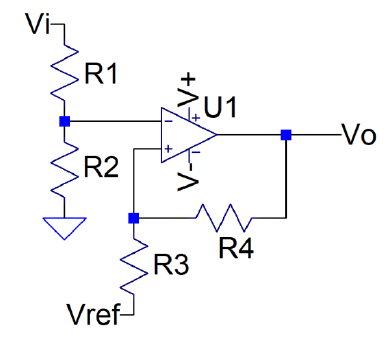
\includegraphics[width=0.70\linewidth]{Secciones/Circuito4/Circuito 4.png}
    \caption{Circuito n° 4}
    \label{fig:Circuito4}
\end{figure}

Los correspondientes valores tensiones de alimentación, referencia y valores de los componentes son los siguientes:

\[V+ = 10V\]
\[V- = 0V\]
\[V_{ref} = 2V\]
\[R_1 = R_2 = R_4 = 10K\Omega\]
\[R_3 = 2K\Omega\]

Se analizan los umbrales de conmutación del circuito. Se consideran las realimentaciones positivas y negativas.

\[v^- = k_1 * V_i\]
\[v^+ = k_2 * (V_o - V_{ref}) + V_{ref}\]
Con:
\[k_1 = \frac{R_2}{R_1 + R_2}\]
\[ k_2 = \frac{R_3}{R_3 + R_4}\]
\subsubsection{Condición \texorpdfstring{$v_d < 0$}{vd < 0}}
Siendo vd = v+ - v-. Si la tensión vd < 0, se considera que en este caso la tensión de salida tiene un valor inicial Vo=Vcc y luego pasa a tener un valor Vo=Vee, debido a la acción de conmutación.  Entonces se tiene:

\[v_d = v^+ - v^- < 0 \Rightarrow V_o = V_{ee}\]
\[v^+ < v^- \]
\[k_2 * (V_o - V_{ref}) + V_{ref} < k_1 * V_i\]
\[\frac{k_2}{k_1} * (V_o - V_{ref}) + \frac{V_{ref}}{k_1} < V_i \]
\[\frac{k_2}{k_1} * V_o + \frac{1 - k_2}{k_1} * V_{ref} < V_i \]
Se tiene:
\[ k_1 = \frac{R_2}{R_1 + R_2} = \frac{10K\Omega}{10K\Omega + 10K\Omega} = 0.5\]

\[ k_2 = \frac{R_3}{R_3 + R_4} = \frac{2K\Omega}{2K\Omega + 10K\Omega} = 0.166\]

Reemplazando en la expresión anterior:

\[\frac{0.166}{0.5} * 10V + \frac{1 - 0.166}{0.5} * 2V < V_i \]
\[3.32V + 3.34V < V_i \]
\[V_i > 6.66V \Rightarrow V_o = V_{cc}\]
Para nuestro caso Vcc= 10V.

\[V_i > 6.66V \Rightarrow V_o = 10V\]

\subsubsection{Condición \texorpdfstring{$v_d > 0$}{vd > 0}}
Se tiene que vd > 0. Previo a esta condición, el circuito tendrá un valor de salida de Vo=Vee, por lo que conmutará de un valor de Vo=Vee a Vo= Vcc. Se desarrolla la condición planteada:
\[v_d = v^+ - v^- > 0 \Rightarrow V_o = V_{cc}\]
\[v^+ > v^-\]

\[ k_2 * (V_o - V_{ref}) + V_{ref} > k_1 * V_i\]

\[\frac{k_2}{k_1} * V_o + \frac{1 - k_2}{k_1} * V_{ref} > V_i \]
Como Vee= 0v, se tiene:
\[\frac{0.166}{0.5} * 0V + \frac{1 - 0.166}{0.5} * 2V > V_i \]
\[\frac{1 - 0.166}{0.5} * 2V > V_i \]
\[V_i < 3.336V \Rightarrow V_o = V_{ee}\]
Para nuestro caso:
\[V_i < 3.336V \Rightarrow V_o = 0V\]

\subsection{Simulación}

\subsubsection{Simulación con alimentación simétrica (Vcc= 10v y Vee= -10v)}

Se realiza la simulación del circuito con alimentación simetrica en el software LTSpice.
\begin{figure}[h!]
    \centering
    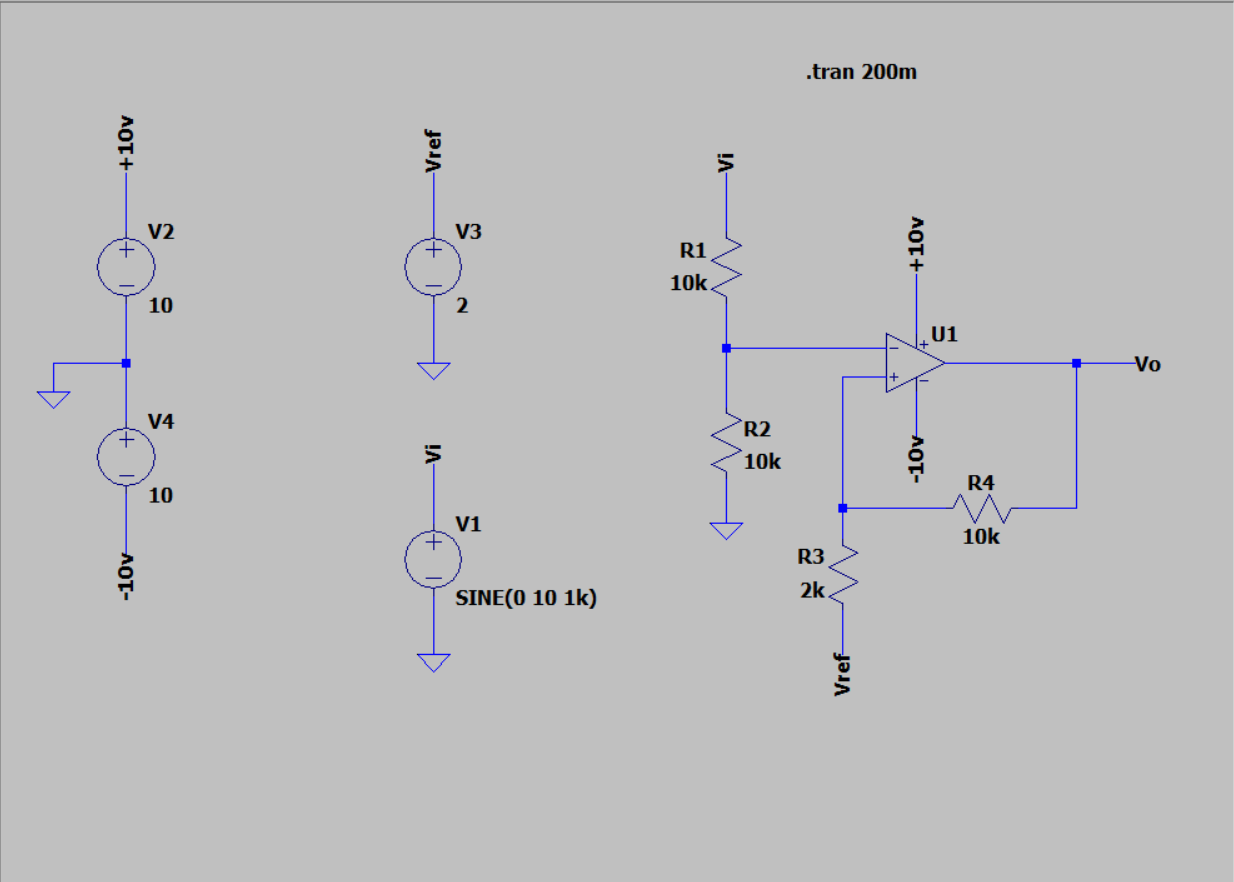
\includegraphics[width=1.0\linewidth]{Secciones/Circuito4/Circuito 4 - Alimentación simétrica.png}
    \caption{Circuito n° 4 - Alimentación simétrica}
    \label{fig:AlimentacionSimetrica}
\end{figure}

Se inyecta una señal senoidal de entrada con las siguientes características:

\[ \widehat{V_i} = 10 \, \text{V} \, (\text{Amplitud pico}) \]
\[frecuency= 1KHz\]

En la siguiente figura se muestra la señal de salida Vo (color verde)  y la señal de entrada Vi (color azul) con los siguientes valores medidos:
\begin{figure}[H]
    \centering
    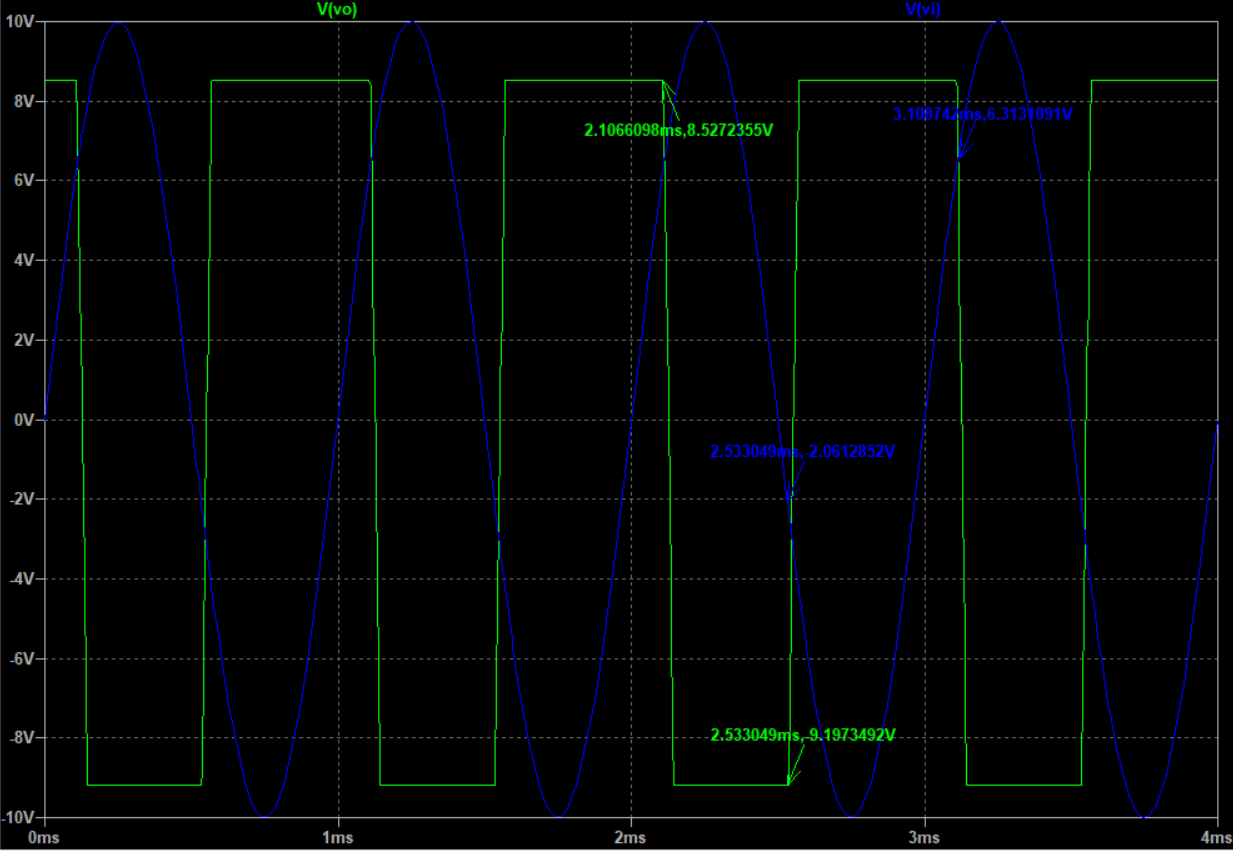
\includegraphics[width=1.0\linewidth]{Secciones/Circuito4/Circuito 4 - Simulación con alimentación simétrica.png}
    \caption{Señal de salida de circuito con alimentación simétrica}
    \label{fig:SimulacionConAlimentacionSimetrica}
\end{figure}

Se observa en la siguiente figura la señal de entrada en el pin v+ (en color azul).

\begin{figure}[H]
    \centering
    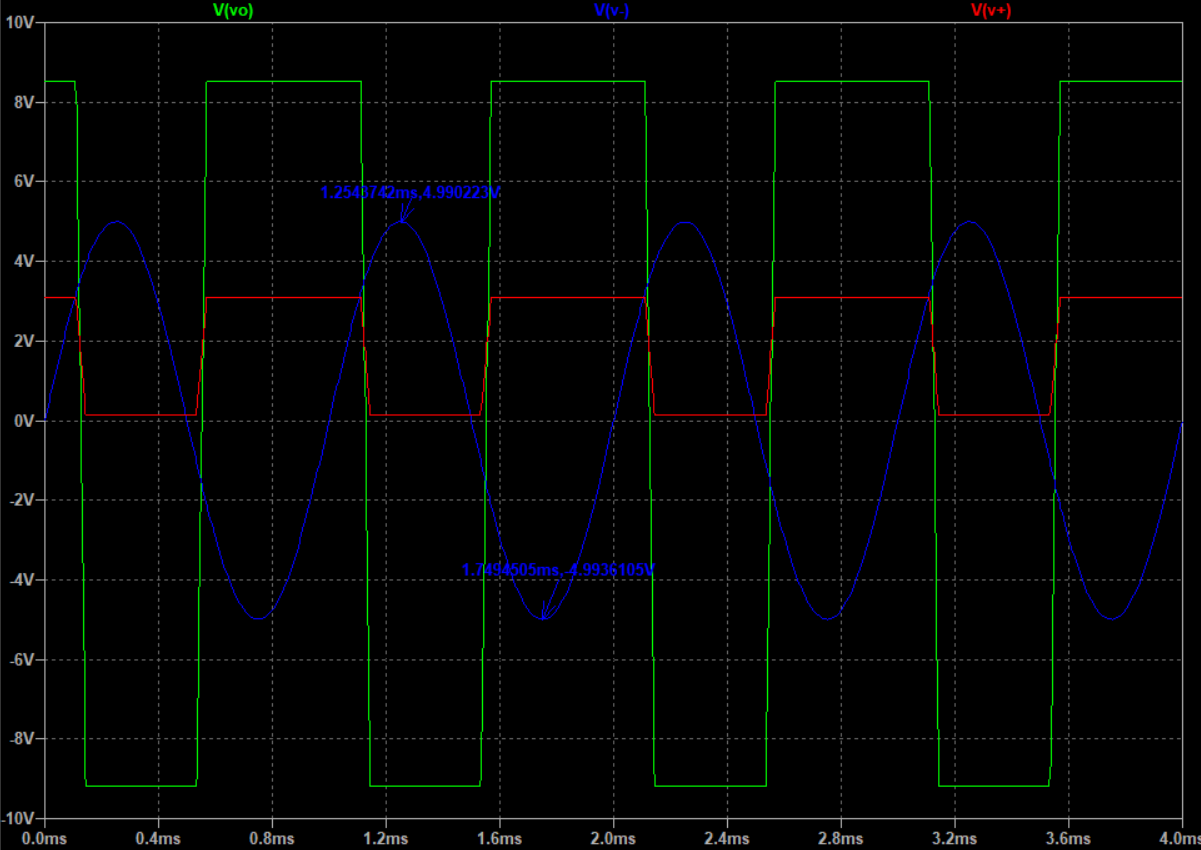
\includegraphics[width=1.0\linewidth]{Secciones/Circuito4/Circuito 4 - Vi no atenuada.png}
    \caption{Señal de entrada en v- sin distorsión}
    \label{fig:ViNoAtenuada}
\end{figure}
- Umbral de conmutación de valor Vo=Vee a Vo=Vcc. 
\[V_{i_{\text{sim}}}= 2.06V\]
Lo cual en teoría se verifica con la condición teórica analizada anteriormente:
\[V_{i_{\text{teórica}}} < 3.336V \Rightarrow \text{con} \; V_{o_{\text{inicial}}} = V_{ee}\]

- Umbral de conmutación de valor Vo= Vcc a Vo= Vee 
\[V_{i_{\text{sim}}}= 6,31V\]
El valor de tensión de umbral de simulación se aproxima al valor teórico de conmutación.
\[V_{i_{\text{teórica}}} > 6.66V \Rightarrow V_{o_{\text{inicial}}}= V_{cc} \]
Se concluye el comportamiento del circuito Schmitt Trigger Inversor, con los siguientes umbrales:

\begin{equation}
    \text{Valores \space de \space conmutación \space =}
    \begin{cases}
      V_{ee} \rightarrow V_{cc}, &  Vi\leq2,06V \\
      V_{cc} \rightarrow V_{ee}, &  Vi\geq6,31V
    \end{cases}
  \end{equation}

Se tiene que los valores reales de la salida difieren de los valores teóricos Vo=Vcc= 10V y Vo=Vee= -10V. Se obtuvieron los siguientes valores de salida Vomáx= 8,53V y Vomín=-9,2V.  Esto es debido a que el amplificador operacional implementado no tiene la característica Rail-to-Rail. 


\subsubsection{Simulación con alimentación asimétrica (Vcc=10V y Vee=0v)}

Se realiza la simulación del circuito con alimentación asimetrica en el software LTSpice.

\begin{figure}[h!]
    \centering
    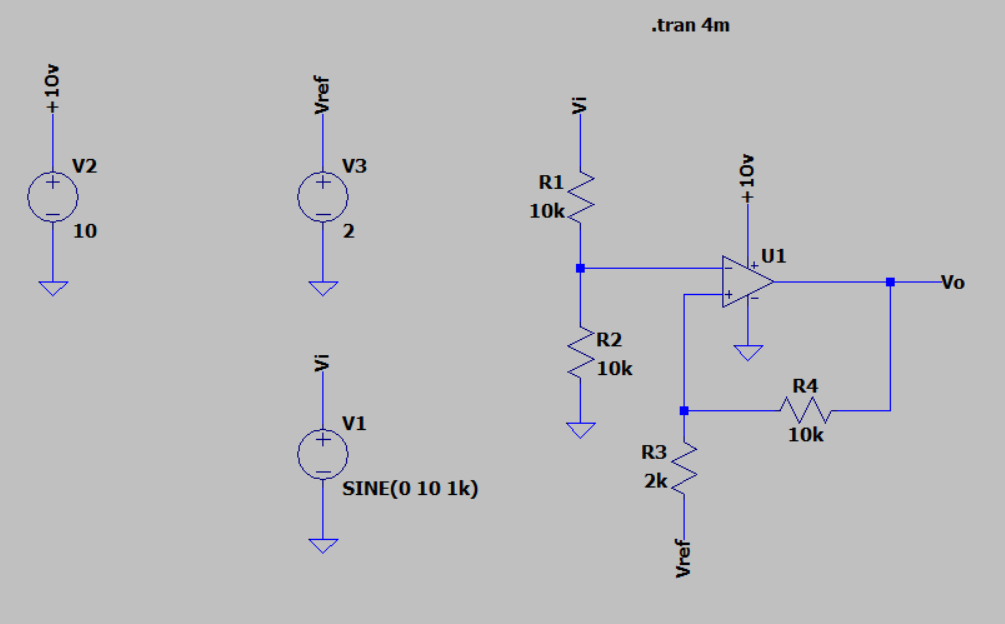
\includegraphics[width=1.0\linewidth]{Secciones/Circuito4/Circuito 4 - Alimentación asimétrica.png}
    \caption{Circuito n° 4 - Alimentación asimétrica}
    \label{fig:AlimentacionAsimetrica}
\end{figure}

Se inyecta una señal senoidal de entrada con las siguientes características:

\[{\widehat{V}}_i= 10v \space (Amplitud \space pico)\]
\[frecuency= 1KHz\]

 En la siguiente figura se muestra la señal de salida Vo (color verde)  y la señal de entrada Vi (color azul). Se obtiene el siguiente comportamiento de la salida del circuito conmutador.
\begin{figure}[h!]
    \centering
    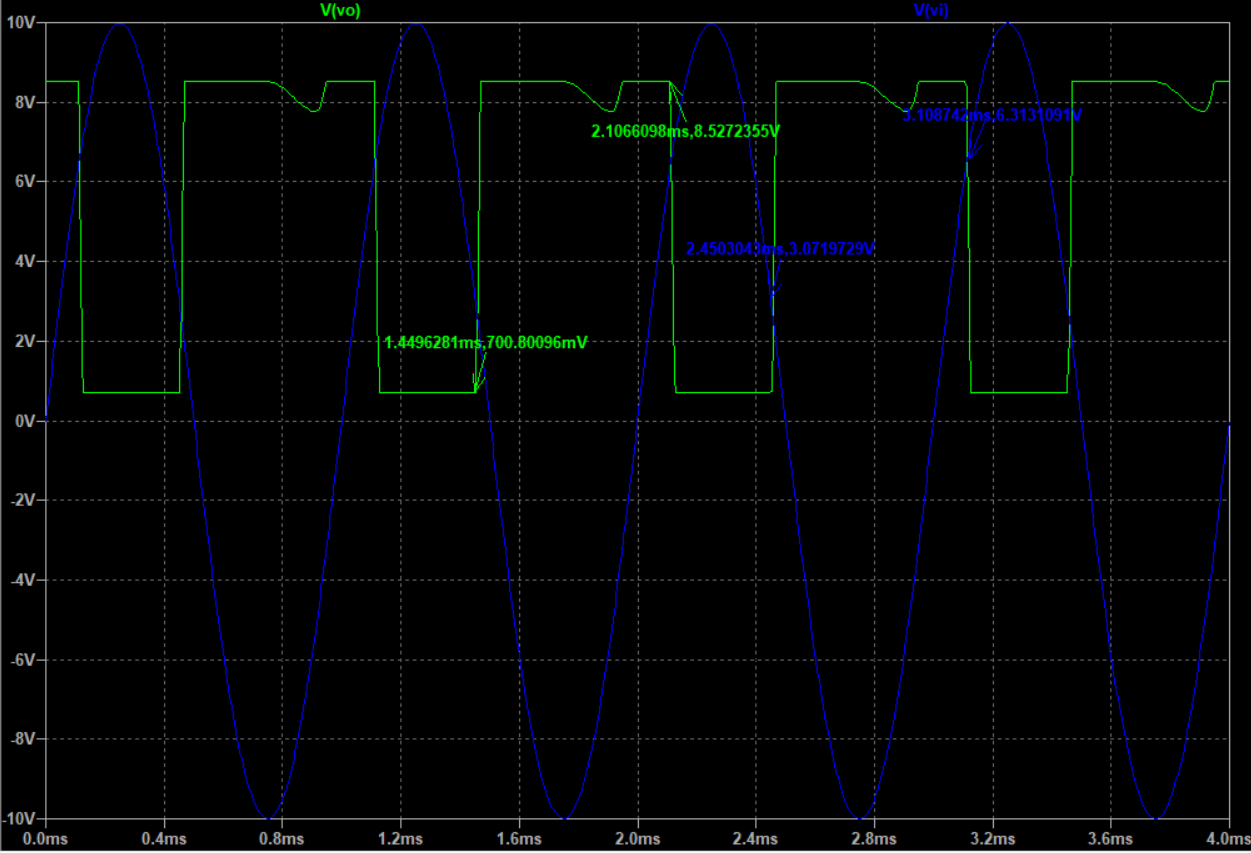
\includegraphics[width=1.0\linewidth]{Secciones/Circuito4/Circuito 4 - Simulación con alimentación asimétrica.png}
    \caption{Señal de salida de circuito con alimentación asimétrica}
    \label{fig:SimulacionConAlimentacionAsimetrica}
\end{figure}
\begin{figure}[h!]
    \centering
    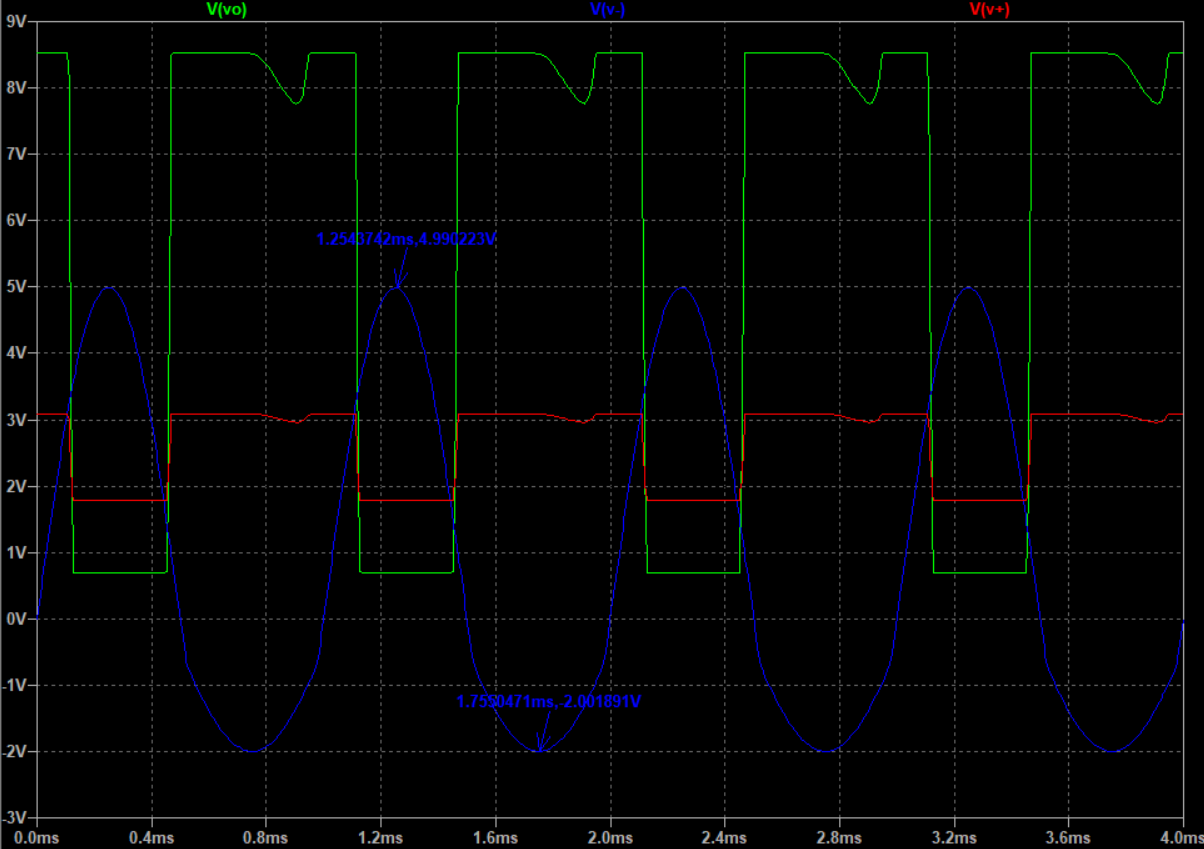
\includegraphics[width=1.0\linewidth]{Secciones/Circuito4/Circuito 4 - Vi atenuada.png}
    \caption{Distorsión de señal de entrada en v-}
    \label{fig:ViAtenuada}
\end{figure}
Se observa en la medición que la señal en el pin v- del amplificador (señal de entrada atenuada) que la misma se distorsiona en el semiciclo negativo. Esto se debe a que los transistores internos que conforman el amplificador operacional no se encuentran polarizados para procesar una señal sinusoidal simétrica.  Esta distorsión no ocurre para el circuito con alimentación simétrica Vcc=10V y Vee=-10V.

Debido a la característica anteriormente nombrada del operacional implementado, se tiene que los valores máximos y mínimos de salida de la simulación difieren de los valores teóricos.

Se obtienen los siguientes valores de tensión de umbral:

- Umbral de conmutación de valor Vo= v- a Vo= v+ 
\[V_{i_{\text{sim}}}= 3,07V\]
Lo cual en teoría se verifica con la condición teórica analizada anteriormente:
\[V_{i_{\text{teórica}}} < 3.336V \Rightarrow con \space V_{o_{\text{inicial}}} = V_{ee}\]
- Umbral de conmutación de valor Vo= v+ a Vo= v- 
\[V_{i_{\text{sim}}}= 6,31V\]

El valor de tensión de umbral de simulación se aproxima al valor teórico de conmutación.
\[V_{i_{\text{teórica}}} > 6.66V \Rightarrow V_{o_{\text{inicial}}}= V_{cc} \]
Se concluye el comportamiento del circuito Schmitt Trigger Inversor propuesto, con los siguientes umbrales para una alimentación asimétrica es la siguiente:

\begin{equation}
    \text{Valores \space de \space conmutación \space =}
    \begin{cases}
      V_{ee} \rightarrow V_{cc}, &  Vi\leq3,07V \\
      V_{cc} \rightarrow V_{ee}, &  Vi\geq6,31V
    \end{cases}
  \end{equation}
  
Se tiene que los valores reales de la salida difieren de los valores teóricos Vo=Vcc= 10V y Vo=Vee= -10V. Se obtuvieron los siguientes valores de salida Vomáx= 8,53V y Vomín=-700mV.  Esto es debido a que el amplificador operacional implementado no tiene la característica Rail-to-Rail. 

Se observa como cambiaría el lazo de histéresis para diferentes valores de Vref.

\begin{figure}[H]
    \centering
    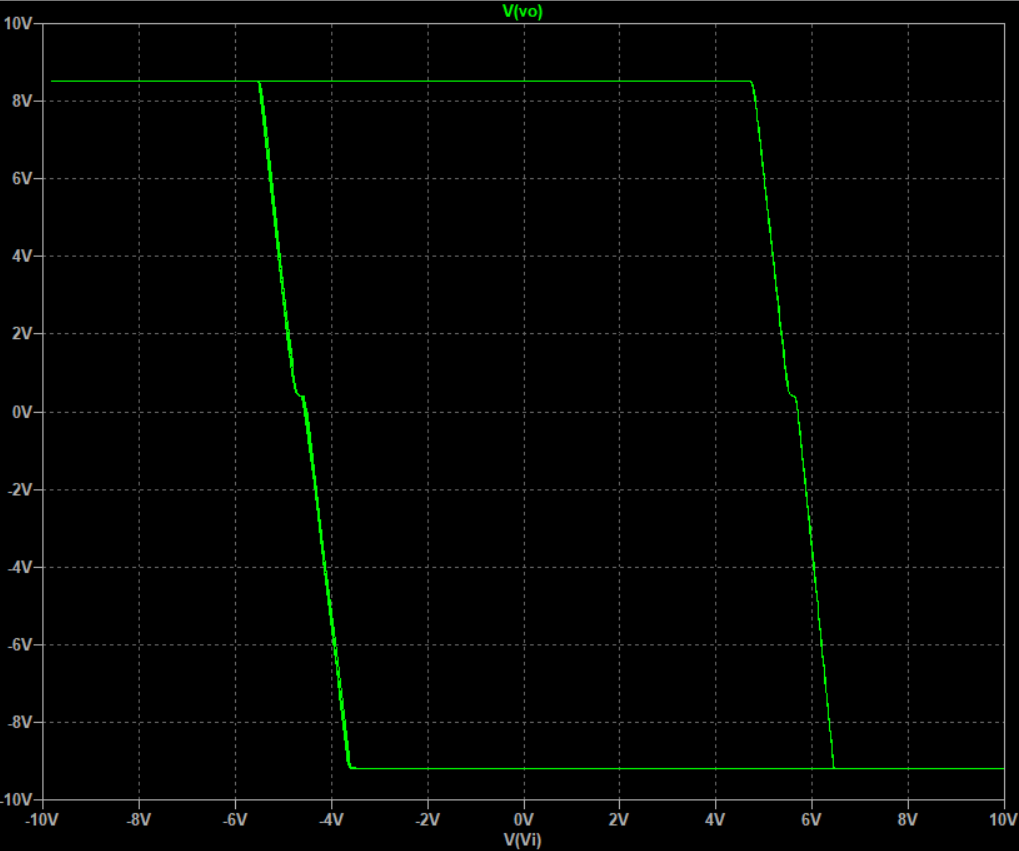
\includegraphics[width=1.0\linewidth]{Secciones/Circuito4/Circuito 4 - Vref1.png}
    \caption{Circuito n° 4 - Ciclo de Histéresis con Vref=1}
    \label{fig:Vref1}
\end{figure}
\begin{figure}[H]
    \centering
    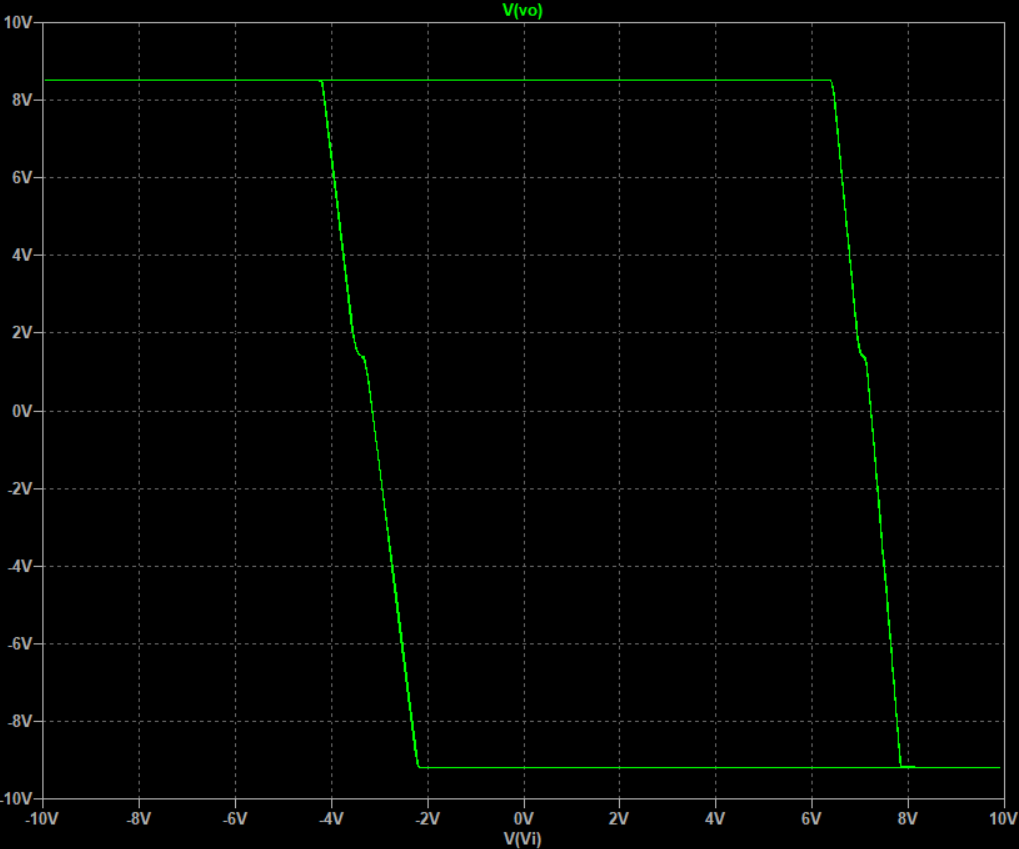
\includegraphics[width=1.0\linewidth]{Secciones/Circuito4/Circuito 4 - Vref2.png}
    \caption{Circuito n° 4 - Ciclo de Histéresis con Vref=2}
    \label{fig:Vref2}
\end{figure}
\begin{figure}[H]
    \centering
    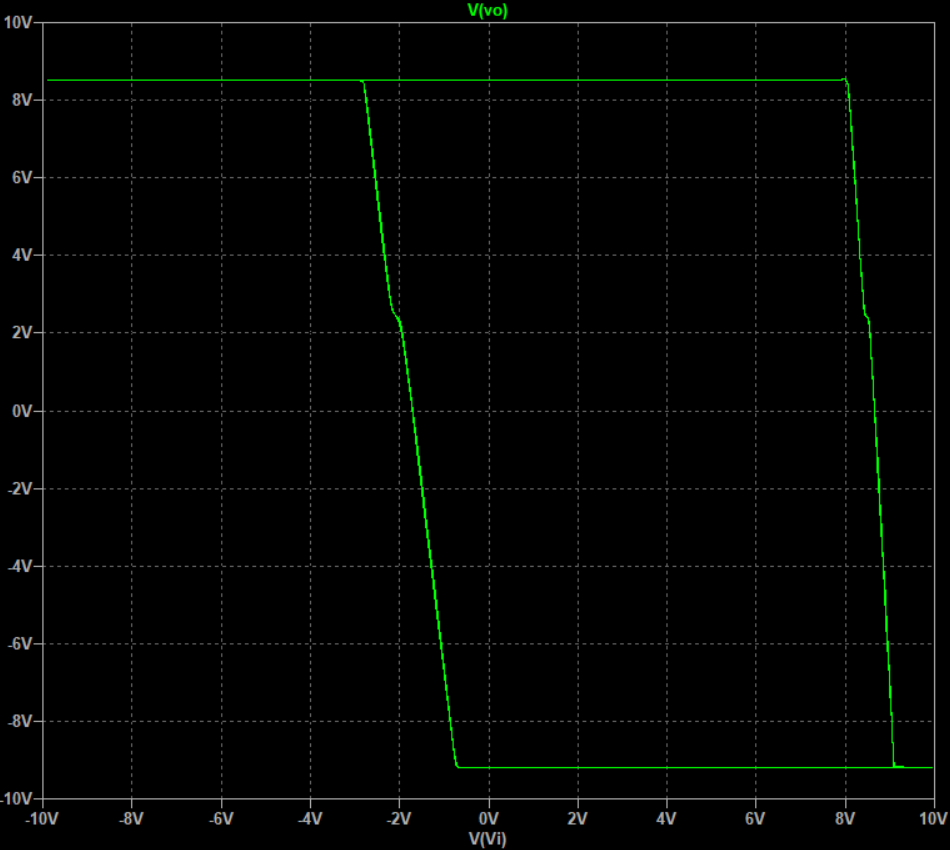
\includegraphics[width=1.0\linewidth]{Secciones/Circuito4/Circuito 4 - Vref3.png}
    \caption{Circuito n° 4 - Ciclo de Histéresis con Vref=3}
    \label{fig:Vref3}
\end{figure}

\begin{figure}[H]
    \centering
    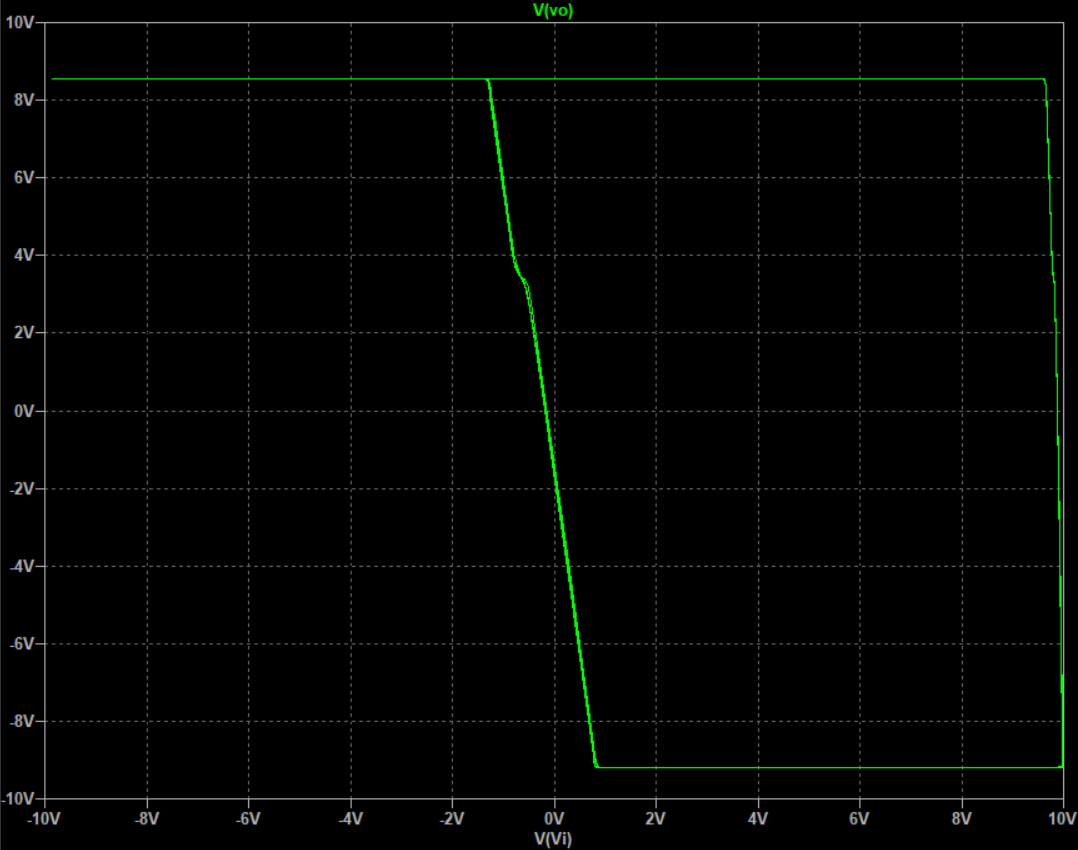
\includegraphics[width=1.0\linewidth]{Secciones/Circuito4/Circuito 4 - Vref4.png}
    \caption{Circuito n° 4 - Ciclo de Histéresis con Vref=4}
    \label{fig:Vref4}
\end{figure}